\section{Matematikken bak trackingen (Vegar)}

	

\section{Tilkobling av kamera til PC (Holger)}

	For \aa \space koble et kamera til en PC og lese dens videobilder trenger man b\aa de maskinvare og programvare. Maskinvaren gir den fysiske tilkoblingen mellom kameraet og PC-en samt gj\o r lavniv\aa s logikk og behandling av dataene. Programvaren abstraherer bort maskinvaren og gir utviklere et brukbart grensesnitt for \aa \space lese og bruke videobildene. Av maskinvare har vi i prosjektet tenkt \aa \space bruke HDMI og et Intensity-kort for \aa \space koble kameraet til PC-en som kj\o rer systemet v\aa rt. Av programvare har vi tenkt \aa \space bruke DirectShow for \aa \space f\aa \space lett tilgang til videobildene fra kameraet.
	
	\subsection{HDMI og Intensity}
	
		HDMI er en standard for et fysisk grensesnitt for \aa \space sende og motta digital lyd og bilde. Apparater med HDMI-kontakt kan kobles til hverandre ved hjelp av en HDMI-kabel (se figur \ref{fig:hdmi}). HDMI er designet for \aa \space h\aa ndtere lyd og bilde med h\o y oppl\o sning, og kan sende opptil 10,2 gigabit per sekund.
		
		\begin{figure}[h]
		\centering
		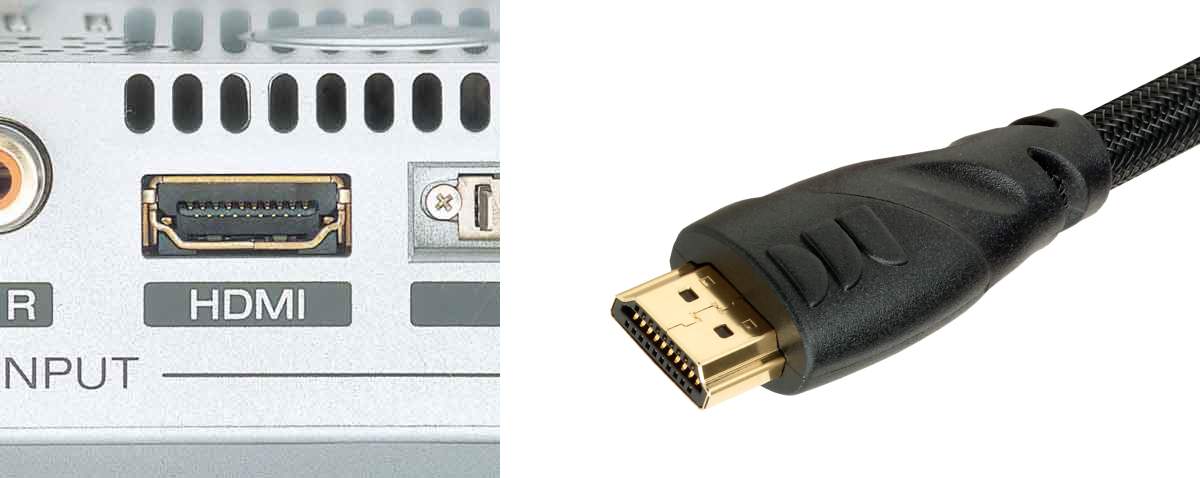
\includegraphics[width=0.60\textwidth]{graphics/hdmi.png}
		\caption{HDMI-kontakt (venstre) og kabel (h\o yre)}
		\label{fig:hdmi}
		\end{figure}
		
		Intensity er et HDMI capture card fra Blackmagic Design. Det er et stykke maskinvare som kan settes inn i en PC for \aa \space gj\o re det mulig \aa \space koble enheter til denne PC-en gjennom HDMI. Kortet kobles til PCI-express-porten i PC-en og har to HDMI-kontaktpunkter: inngang og utgang (se figur \ref{fig:intensity}).
		
		\begin{figure}[h]
		\centering
		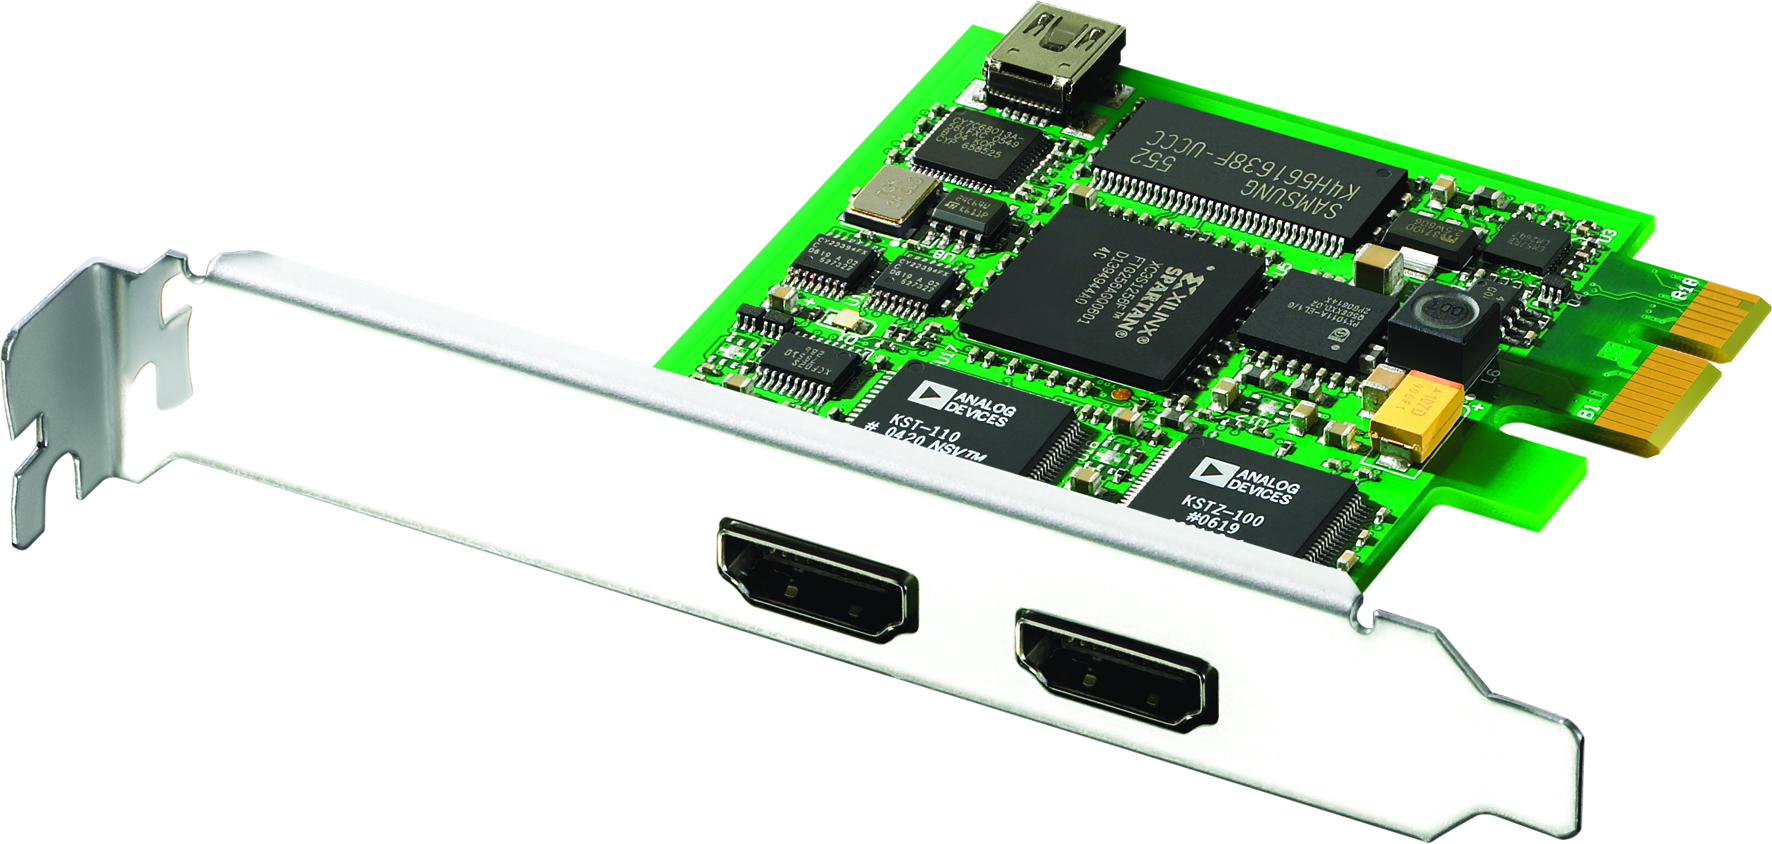
\includegraphics[width=0.60\textwidth]{graphics/intensity.png}
		\caption{Intensity fra Blackmagic Design}
		\label{fig:intensity}
		\end{figure}
	
	\subsection{DirectShow}
	
		DirectShow er et rammeverk og programvaregrensesnitt for \aa \space h\aa ndtere multimedia p\aa \space PC-er. Det er utviklet av Microsoft og gj\o r det mulig \aa \space spille av og ta opp media (typisk lyd og/eller bilde) gjennom et felles grensesnitt, og abstraherer bort maskinvaren. Bildene fra videokamera koblet til et Intensity-kort er tilgjengelig gjennom DirectShow. DirectShow er tilgjengelig gratis fra Microsofts nettsider.

\section{\AA \space spore punkter i et bilde (Holger)}

	